\section{Method}
\label{sec:method}

We formulate context-enriched field as a minimal context-aware enrichment of a
geometry-only port-Hamiltonian navigator. The goal is to let local
context reshape the closed-loop field: activating risk preferences,
barriers, and motion directions only when they are relevant. We first
define the local-risk interface, then introduce the shared
$(\Pos,\Mom)$ update and the context-energy term that produces the new
force channel.

\subsection{Problem setup: local information, latent risk}
\label{sec:method:setup}

At time $t$, the agent observes only local information: the goal
displacement $\vec c_g-\vec c_t$, nearby obstacle or neighbor features
$\{(C_j,R_j,W_j)\}_{j=1}^{N(t)}$ within sensing radius $\hat d$, and a
$P\times P$ context patch $P_t$ centered at its current position. The
patch contains a smoothed risk field $\tilde r(\cdot)\in[0,1]$ and a
signed-distance field $\phi(\cdot)$ to hard hazards or infeasible
regions. The risk field may represent terrain material, traffic
interaction risk, or any locally queryable context; we require only that
it be differentiable after smoothing. At each integration step, $P_t$ is
bilinearly resampled at the current position, so forces and costs are
computed along the realized trajectory. All methods are evaluated under
the same local-information contract.

Each observation therefore defines a local optimization instance: goal
attraction, clearance barriers, soft risk, hard hazards, and lateral
motion may all be available, but only some should be active. We use \textit{action-space adaptation} in this restricted continuous sense: the
learner does not enumerate discrete actions, but changes which force
channels have non-negligible magnitude under the sensed context.

\paragraph{Static and dynamic risk.}
The same interface covers both static and dynamic settings. In DFC and
RELLIS, $\tilde r$ and $\phi$ are fixed semantic/material fields, so risk
depends on the path taken through the map. In highway-env, the local
patch changes as neighboring vehicles move, close gaps, or block lateral
escape. Thus static domains test material-aware path selection, while
dynamic domains test whether the learned field preserves clearance,
time-to-collision, and maneuvering room before violations become
terminal.

% ----------------------------------------------------------------------
\subsection{The shared $(\Pos,\Mom)$-update skeleton}
\label{sec:method:skeleton}
% ----------------------------------------------------------------------

The geometry-only and context-aware learners share an identical
phase-space update structure. Written side by side, with $\tau$ the
integration step, $\Mass$ the (constant) mass matrix, and $R_\theta$
the learned dissipative port:
\begin{equation}
\renewcommand{\arraystretch}{1.6}
\begin{array}{ll}
\textbf{Geom. scaffold (geometry-only)} & \textbf{Ctx-enriched (context-aware)} \\[2pt]
\Mom_{t+1} = \Mom_t
  - \tau\,\nabla_\Pos \Ham_{\mathrm{geom}}
  - \tau R_\theta(\Mom_t)
&
\Mom_{t+1} = \Mom_t
  - \tau\,\nabla_\Pos \Ham_{\mathrm{geom}}
  \;\boldsymbol{-\,\tau\,\nabla_\Pos \Ham_{\mathrm{ctx}}}
  - \tau R_\theta(\Mom_t) \\[6pt]
\Pos_{t+1} = \Pos_t + \tau \Mass^{-1} \Mom_{t+1}
&
\Pos_{t+1} = \Pos_t + \tau \Mass^{-1} \Mom_{t+1}
\end{array}
\label{eq:method:skeleton}
\end{equation}
The $\Pos$-update is identical. The dissipative port is identical. The
geometric force is identical and is carried forward unchanged. The
\emph{only} dynamical difference is the boldfaced term
$-\tau\,\nabla_\Pos \Ham_{\mathrm{ctx}}$ in the context-enriched field $\Mom$-update.
This is the entire structural content of the paper: a single new term,
and its consequences. The remainder of this section traces those
consequences.

A consequence already visible in Eq.~\eqref{eq:method:skeleton}: new
sensory information enters through $\Mom$, not through an external
critic or replanner. The cotangent variable acts as the internal
evaluator that integrates clearance, material risk, and dissipative
correction into a single force balance. The decision field \emph{is}
the policy.

% ----------------------------------------------------------------------
\subsection{Factored stored energy and force channels}
\label{sec:method:energy}
% ----------------------------------------------------------------------

The context-enriched field stored energy decomposes additively as
\begin{equation}
\Ham_\theta(\Pos, \Mom)
\;=\;
\underbrace{\tfrac{1}{2}\Mom^{\!\top}\Mass^{-1}\Mom}_{\Ham_{\mathrm{kin}}}
\;+\;
\underbrace{\beta\, D_{\mathcal{G}}(\Pos, \vec c_g)
            + \textstyle\sum_j \alpha_j\, b_{\mathrm{IPC}}(d_j)}_{\Ham_{\mathrm{geom}}\;\text{(Geom. scaffold)}}
\;+\;
\underbrace{\lambda_s\,\tilde r(\vec c)
            + \lambda_h\, b_{\mathrm{sp}}\!\bigl(\phi(\vec c)\bigr)}_{\Ham_{\mathrm{ctx}}\;\text{(new in Ctx-enriched)}},
\label{eq:method:energy}
\end{equation}
where $b_{\mathrm{IPC}}$ is the incremental potential contact
barrier~\citep{li2020ipc} on per-obstacle clearance $d_j$, and
$b_{\mathrm{sp}}(\phi) = k^{-1}\log(1 + \exp(k(\hat d_\phi - \phi)))$
is a softplus-relaxed inverse SDF activated only when $\phi < \hat
d_\phi$. The dissipative port $R_\theta(\Pos, \Mom) = \gamma \Mass^{-1}
\Mom$ remains structurally separate from the stored
energy~\citep{vanderschaft2014port}, allowing symplectic and dissipative
parts of the field to be analyzed independently. In our experiments
$\Mass = I$, so $\Mass^{-1}\Mom = \Mom$ in code; we keep $\Mass$
explicit in the formalism for general port-Hamiltonian compatibility.
We use the subscript ``ctx'' to emphasize that the same term supports
material contexts in DFC and interaction contexts in highway-env; the
mechanism is the context-conditioned force, not the source of the risk
field.

\begin{figure}[t]
  \centering
  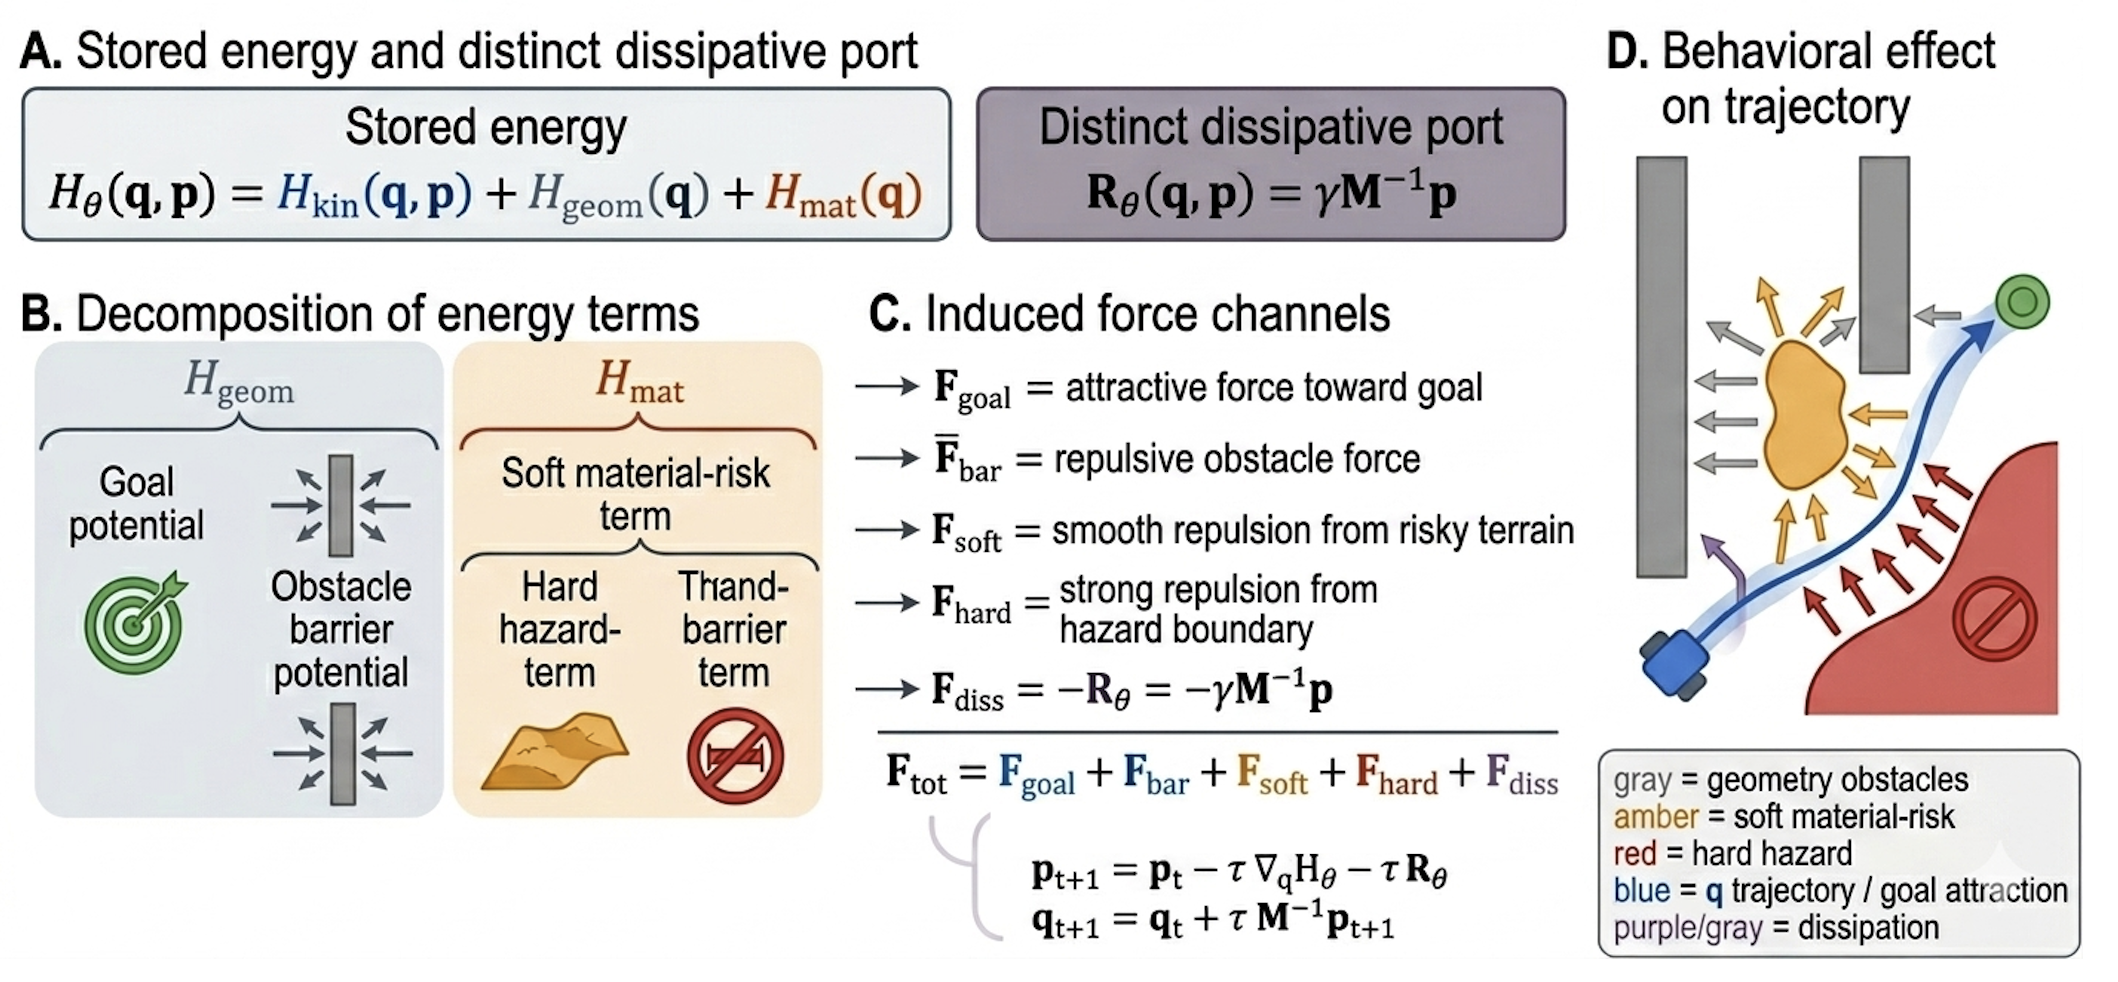
\includegraphics[width=\linewidth]{figures/ch4_factored_hamiltonian.png}
  \caption{\textbf{Factored stored energy and induced force channels.}
  \emph{(A)} The context-enriched energy $\Ham_\theta$ decomposes additively into
  kinetic, geometric, and context components; the dissipative port
  $R_\theta$ remains structurally separate. \emph{(B)} The geometric
  energy carries goal-attraction and obstacle-barrier potentials; the
  context energy carries soft-risk and hard-hazard terms.
  \emph{(C)} Each potential induces a force channel: $F_{\mathrm{soft}}
  = -\lambda_s \nabla\tilde r$ deflects the trajectory smoothly toward
  lower-risk lanes; $F_{\mathrm{hard}} = -\lambda_h\,
  b_{\mathrm{sp}}'(\phi)\,\nabla\phi$ acts as a soft barrier that
  strengthens sharply near hazard boundaries while remaining
  differentiable. \emph{(D)} The field shifts the agent toward the
  lower-risk feasible maneuver \emph{when one exists}, and remains
  near-static otherwise when the local feasibility gate closes
  (see the route-aware context-force paragraph below). Neither channel exists in
  geometry scaffold, and neither can be obtained by reweighting the geometric
  coefficients. Formally, if $\nabla\tilde r(q)$ has a component outside
  the span of the geometry-scaffold force dictionary, no reweighting of
  geometry-scaffold coefficients can reproduce $F_{\mathrm{soft}}$; see
  Appendix~\ref{app:force_dictionary_separation}.}
  \label{fig:method:factored}
\end{figure}

Differentiating $\Ham_{\mathrm{ctx}}$ yields two qualitatively distinct
force channels:
\begin{equation}
F_{\mathrm{ctx}}(\vec c)
\;=\;
\underbrace{-\lambda_s\,\nabla \tilde r(\vec c)}_{F_{\mathrm{soft}}\,:\;\text{lateral deflection}}
\;+\;
\underbrace{-\lambda_h\, b_{\mathrm{sp}}'(\phi(\vec c))\,\nabla\phi(\vec c)}_{F_{\mathrm{hard}}\,:\;\text{hazard repulsion}},
\qquad
b_{\mathrm{sp}}'(\phi) \;=\; -\sigma\!\bigl(k(\hat d_\phi - \phi)\bigr).
\label{eq:method:force}
\end{equation}
The two channels have different regularity. $F_{\mathrm{soft}}$ is a
smooth gradient field acting wherever $\tilde r$ varies; it expresses
preference among feasible maneuvers. $F_{\mathrm{hard}}$ approaches a
step function as $\phi \to 0^+$; it expresses a near-prohibition on
boundary contact, smoothed enough to remain differentiable. Risk does
not enter the algorithm as a cost evaluated after the fact; it enters
as a force that reshapes the dynamics directly.

\paragraph{Contextual objective and action degrees of freedom.}
Eq.~\eqref{eq:method:energy} also clarifies how the objective and
constraint set change with context. The geometric term supplies a
goal-and-clearance scaffold. The soft context term supplies a
reward-like preference over safer feasible directions. The hard hazard
term supplies a constraint-like barrier whose active set changes with
the local SDF. The force decomposition turns these terms into an
effective action product space: longitudinal acceleration and damping,
lateral deflection, obstacle repulsion, and hazard avoidance. The context-enriched field
learns coefficients for this product space, but the sensed gradients
determine which factors can actually act. Thus moving objects and
changing material patches do not require the learner to search all
actions uniformly; they modulate which coarse degrees of freedom are
available and useful in the current scene.

The operational objective can be summarized as a balanced failure-profile
cost,
\begin{equation}
\mathcal{J}_{\mathrm{bal}}(\pi)
=
\lambda_{\mathrm{goal}}C_{\mathrm{goal}}
+\lambda_{\mathrm{risk}}C_{\mathrm{risk}}
+\lambda_{\mathrm{barrier}}C_{\mathrm{barrier}}
+\lambda_{\mathrm{control}}C_{\mathrm{control}}
+\lambda_{\mathrm{smooth}}C_{\mathrm{smooth}}
+\lambda_{\mathrm{dyn}}C_{\mathrm{dyn}},
\label{eq:method:balanced_objective}
\end{equation}
where the final dynamic-risk term is active for interaction domains such
as highway-env. The terms are not meant to be optimized independently:
low risk by stopping, low control by failing to evade, and short paths
through hazards are all bad solutions. The purpose of the context-enriched field is to
learn a context-conditioned compromise among these terms in the induced
continuous vector field.

These terms map directly to the evaluation profile: goal/progress maps
to success, progress, and path length; soft risk maps to cumulative risk,
risk density, and CVaR; barriers map to hard-hazard length, off-road
events, and lane violations; control and smoothness map to force effort,
hard braking, oscillation, curvature, and jerk; dynamic risk maps to
clearance, TTC violation, and intervention-window diagnostics. This
one-to-one mapping is deliberate: the metrics are not post-hoc
decorations, but measurements of the same terms the learned field is
balancing.

\paragraph{Route-aware context force.}
Eq.~\eqref{eq:method:force} is the scalar context-enriched force: it follows the
local risk gradient wherever the smoothed material field changes. In
off-road scenes this is sometimes too reactive. A low-risk-looking patch may
be separated by a fence, berm, vehicle, or non-traversable boundary; pushing
toward that patch is precisely the false activation measured in R2. For
RELLIS and other local-BEV domains we therefore use a route-aware variant of
the same context Hamiltonian:
\begin{equation}
F_{\mathrm{ctx}}^{\mathrm{ra}}(\vec c;P_t)
=
m_{\mathrm{feas}}(\vec c,z_t)
\bigl(-\lambda_s \nabla \tilde r(\vec c)\bigr)
-\lambda_h\, b_{\mathrm{sp}}'(\phi(\vec c))\,\nabla\phi(\vec c),
\label{eq:method:route_aware_force}
\end{equation}
where $z_t$ denotes the finite set of local candidate rollouts sampled from
the current BEV patch $P_t$. The scalar risk force and hard-hazard barrier
are unchanged; the only added object is
$m_{\mathrm{feas}}\in[0,1]$, a local affordance gate that determines whether
the soft-risk force is allowed to act.

The gate is computed from the same local patch available to all
local-sensing methods. From the current state we roll out $K$ short-horizon
motion primitives $\{\xi_k\}_{k=1}^K$ inside the sensed BEV window and compute
\begin{equation}
R_k=\int_{\xi_k}\tilde r(s)\,ds,\qquad
C_k=\min_{\xi_k}\phi(s),\qquad
I_k=\mathbf{1}[C_k>\delta_\phi\ \text{and}\ \xi_k\subset\mathcal{T}(P_t)],
\end{equation}
where $\mathcal{T}(P_t)$ is the traversable mask induced by the local
semantics. Let $k^\star$ be the feasible candidate with lowest soft-risk
exposure, and let $k_{\mathrm{scaf}}$ be the candidate closest to the geometry scaffold
scaffold direction. We use the soft gate
\begin{equation}
m_{\mathrm{feas}}(\vec c,z_t)
=
\sigma\!\left(\kappa_R
\left[(R_{k_{\mathrm{scaf}}}-R_{k^\star})-\rho_R\right]\right)
\,
\sigma\!\left(\kappa_C(C_{k^\star}-\delta_\phi)\right)
I_{k^\star}.
\label{eq:method:route_gate}
\end{equation}
Thus the soft-risk force activates only when a locally feasible candidate
reduces risk by a margin; it is suppressed when the apparent lower-risk
region is blocked, outside the traversable mask, or absent. During one
Hamiltonian integration substep $m_{\mathrm{feas}}$ is treated as the
locally measured context coefficient, exactly like the coefficients
predicted from the risk patch. Equivalently, the substep uses the local
energy $H_{\mathrm{ctx}}^{\mathrm{ra}}=
m_{\mathrm{feas}}\lambda_s\tilde r+
\lambda_h b_{\mathrm{sp}}(\phi)$, with the affordance coefficient frozen
until the next BEV update.

This definition is important for the interpretation of the experiments.
The route-aware context-enriched field is not an oracle over the global route and it is not a
full-map planner hidden inside the policy. It uses only the local BEV patch,
the local SDF, and finite-horizon candidate rollouts within the same sensing
radius used by the local planner baselines. The R1/R2/R3 labeling procedure is
separate from the method: it is used to score whether activation was correct,
not to provide a global path to the policy.

\paragraph{Coefficient prediction.}
The new coefficients $(\lambda_s, \lambda_h)$ are predicted by
sigmoid-bounded heads from a CNN encoding of the risk patch $P_t$
fused with the existing goal-context token; the geometric heads
$(\alpha,\beta,\gamma)$ are unchanged. Freezing the geometry scaffold geometry
heads makes the new coefficients the only route by which context can
alter the field, which is what makes the ablations interpretable.
Thus the policy learns not only a trajectory predictor, but also
context-conditioned weights in front of the risk and barrier terms. In
highway-env we additionally expose a contextual lateral response
coefficient and a TTC-conditioned interaction channel; in boxed traffic
these terms are suppressed by the local affordances, while in the open
slow-leader case they activate.
These learned coefficients are distinct from the fixed weights used only
to report aggregate evaluation scores.

% ----------------------------------------------------------------------
\subsection{Tail-risk objective: well-posed differentiation through the quantile}
\label{sec:method:cvar}
% ----------------------------------------------------------------------

The episodic cost combines a terminal goal error, true rollout arc
length, cumulative soft-risk exposure, and a hard-hazard step count:
\begin{equation}
J(\theta) \;=\;
w_g\,\|\Pos_T{-}\Pos_g\|^2
\;+\; w_\ell\,\sum_t \|\Pos_{t+1}{-}\Pos_t\|
\;+\; w_r\,\sum_t \tilde r(\Pos_t)\,\|\Pos_{t+1}{-}\Pos_t\|
\;+\; w_h\,\sum_t \mathbf{1}\!\bigl[\phi(\Pos_t) < \epsilon\bigr],
\label{eq:method:J}
\end{equation}
each rollout realized by integrating Eq.~\eqref{eq:method:skeleton} for
$H$ steps. We use the true rollout arc length rather than $\tau H$ as
the length proxy, so that detoured paths are correctly penalized.

\paragraph{Why expected cost is insufficient.}
Catastrophic contact, collision, or route failure is a tail event: the
bulk of rollouts may look acceptable while the failures that determine
deployment safety are rare. Expected-cost training is then dominated by
typical-case path quality and allocates too little gradient to the
rollouts where new context force channels must become active.

\paragraph{Tail-risk objective and well-posed gradient.}
We instead optimize $\cvar{\alpha}[J] = \mathbb{E}[J \mid J \geq
\mathrm{VaR}_\alpha(J)]$, the conditional mean of the worst $1{-}\alpha$
fraction of rollouts. Direct differentiation is awkward because
$\mathrm{VaR}_\alpha(J)$ is a non-smooth functional of a
$\theta$-dependent distribution. We use the Rockafellar–Uryasev
variational form~\citep{rockafellar2000optimization}:
\begin{equation}
\cvar{\alpha}\!\bigl[J(\theta)\bigr]
\;=\;
\min_{\eta \in \mathbb{R}}\;
\bigl\{\,\eta + \tfrac{1}{1-\alpha}\,
\mathbb{E}[(J(\theta) - \eta)_+]\bigr\},
\label{eq:method:cvar_var}
\end{equation}
At the minimizing threshold $\eta^*$, the envelope theorem gives the
gradient with respect to $\theta$ while holding $\eta^*$ fixed. This
justifies the empirical estimator
\begin{equation}
\widehat{\cvar{\alpha}}(\theta)
\;=\;
\hat\eta + \frac{1}{(1-\alpha)\,B}\sum_{i=1}^B \bigl(J^{(i)}(\theta) - \hat\eta\bigr)_{+},
\qquad
\hat\eta = \widehat{Q}_\alpha(\{J^{(i)}\}_{i=1}^B),
\label{eq:method:cvar_emp}
\end{equation}
with $\hat\eta$ \emph{detached from the computation graph}.
Backpropagation produces the Rockafellar–Uryasev sample subgradient:
gradient flows only through the $\lceil(1-\alpha)B\rceil$ rollouts that
exceed the empirical quantile, giving a consistent estimator of the
population subgradient under mild regularity~\citep{hong2014monte}. We use
$\alpha = 0.95$, $B = 64$, concentrating each gradient step on the
worst $\sim 3$ rollouts. The role of CVaR here is therefore not just
a different scalarization of the same loss: it routes gradient
through the new force channel exactly on the rollouts where that
channel matters. On those rollouts, $-\tau\nabla\tilde r$ contributes
a non-zero $\partial \Pos_{t+1}/\partial \lambda_s$ at every step,
driving $\lambda_s$ toward values that bias the field away from
high-risk regions or interactions \emph{exactly where the safety signal lives}.

% ----------------------------------------------------------------------
\subsection{Three loops as three computational jobs}
\label{sec:method:loops}
% ----------------------------------------------------------------------

The context-enriched field uses three nested update loops operating at different
timescales: a segment-level coefficient corrector, an episode-level
CVaR backpropagation loop, and a curriculum advancement loop. These
loops update different objects from different information sources, so
the main text treats them as the computational interface between the
Hamiltonian force channels and training. The full loop diagram,
implementation details, and consolidated training algorithm are given in
Appendix~\ref{app:ctx_loops_hierarchy}.

% ----------------------------------------------------------------------
\subsection{The enrichment principle}
\label{sec:method:enrichment}
% ----------------------------------------------------------------------

Sections~\ref{sec:method:skeleton}--\ref{sec:method:loops} construct
The context-enriched field by adding one context energy to the shared Hamiltonian update.
The important consequence is not merely that the derivative of this
energy is a force, but that the force has testable selectivity
implications.

\begin{proposition}[Selectivity consequences of context-energy enrichment]
\label{prop:enrichment}
Let the geometry scaffold and context-enriched field share the same geometric Hamiltonian,
dissipative port, mass matrix, and integration rule, and let
\(\Ham^{(2)}=\Ham^{(1)}+\Ham_{\mathrm{ctx}}\) with
\(F_{\mathrm{ctx}}=-\nabla_{\Pos}\Ham_{\mathrm{ctx}}\). Under the
boundedness and local Lipschitz assumptions stated in
Appendix~\ref{app:theory}, the following consequences hold.
\textbf{Corollary 1 (scaffold preservation):} if the context gate closes
or the context coefficients vanish so that
\(\sup_t\|F_{\mathrm{ctx}}(q_t)\|\le\varepsilon\), then the context-enriched field
rollout remains within \(O(\varepsilon)\) of the geometry-scaffold rollout over a
finite horizon. \textbf{Corollary 2 (no hallucinated escape):} if the
lateral projection satisfies
\(\sup_t\|P_\perp F_{\mathrm{ctx}}(q_t)\|\le\varepsilon_\perp\), then
the lateral deviation from the scaffold is bounded by
\(O(\varepsilon_\perp)\). \textbf{Corollary 3 (risk deflection):} if a
feasible lateral direction has projected risk-gradient margin
\(\Delta\) and projected hard-barrier forces cancel the soft-risk force
by at most \(\chi\), then
\(\|P_\perp F_{\mathrm{ctx}}\|\ge\lambda_s\Delta-\chi\), and one
semi-implicit step decreases local soft risk relative to the scaffold by
\(O(\tau^2\lambda_s\Delta^2)\) when \(\lambda_s\Delta>\chi\).
\end{proposition}

The full statements and proofs are given in
Appendix~\ref{app:theory}: channel creation in
Lemma~\ref{lem:enrichment_channels}, scaffold preservation in
Theorem~\ref{thm:scaffold_preservation}, no hallucinated lateral escape
in Corollary~\ref{cor:no_hallucination}, and risk deflection in
Theorem~\ref{thm:risk_deflection}. Table~\ref{tab:method:theory_metrics}
shows how these consequences are falsified empirically.

\begin{table}[t]
\centering
\caption{\textbf{Theory-to-metric map.} Each consequence of
context-energy enrichment predicts a directly measured quantity in
Section~\ref{sec:experiments}.}
\label{tab:method:theory_metrics}
\begin{tabular}{p{0.47\linewidth}p{0.42\linewidth}}
\toprule
Theoretical consequence & Experimental metric \\
\midrule
Energy enrichment creates a distinct context-force channel
& Force decomposition and force-risk alignment \\
Scaffold preservation when \(F_{\mathrm{ctx}}\) is small or gated off
& R3 scaffold preservation error (SPE) \\
No hallucinated escape when \(P_\perp F_{\mathrm{ctx}}\) is small
& R2 false activation rate (FAR) and lateral deviation \\
Risk deflection under projected risk-gradient margin
& R1 correct activation rate (CAR) and risk reduction \\
\bottomrule
\end{tabular}
\end{table}

This is the operational meaning of the enrichment principle: the same
Hamiltonian term that introduces the force channel also determines when
that channel can be active, when it must remain small, and which
mechanistic metric should expose failure if the implementation violates
the theory.
